\documentclass{article}

\newcommand{\ep}{\rule{.06in}{.1in}}
\textheight 9.5in

\usepackage{amssymb, bm}
\usepackage{amsmath}
\usepackage{amsthm}
\usepackage{graphicx, subcaption, booktabs}
\graphicspath{{/Users/andrewwork/thesis/jump-velocity/plots/}}

\usepackage{tikz, pgfplots, pgfplotstable, chemfig, xcolor}

% \usepgfplotslibrary{colorbrewer, statistics}
% \pgfplotsset{
%   exact axis/.style={grid=major, minor tick num=4, xlabel=$v^*$,
%     legend entries={PDF, CDF},},
%   every axis plot post/.append style={thick},
%   table/search
%   path={/Users/andrewwork/thesis/jump-velocity/dat-files},
%   colormap/YlGnBu,
%   cycle list/Set1-5,
%   legend style={legend cell align=left,},
% }

% \usepgfplotslibrary{external}
% \tikzexternalize

\renewcommand{\arraystretch}{1.2}
\pagestyle{empty} 
\oddsidemargin -0.25in
\evensidemargin -0.25in 
\topmargin -0.75in 
\parindent 0pt
\parskip 12pt
\textwidth 7in
%\font\cj=msbm10 at 12pt

\newcommand{\tn}{\textnormal}
\newcommand{\stiff}{\frac{k_f}{\gamma}}
\newcommand{\dd}{d}
\newcommand{\Der}[2]{\frac{\dd #1}{\dd #2}}
\newcommand{\Pder}[2]{\frac{\partial #1}{\partial #2}}
\newcommand{\Integral}[4]{\int_{#3}^{#4} {#1} \dd #2}
\newcommand{\vect}[1]{\boldsymbol{\mathbf{#1}}}
\newcommand{\mat}[1]{\underline{\underline{#1}}}
\DeclareMathOperator{\Exp}{Exp}

% Text width is 7 inches

\def\R{\mathbb{R}}
\def\N{\mathbb{N}}
\def\C{\mathbb{C}}
\def\Z{\mathbb{Z}}
\def\Q{\mathbb{Q}}
\def\H{\mathbb{H}}
\def\B{\mathcal{B}} 
%\topmargin -.5in 

\setcounter{secnumdepth}{2}
\begin{document}
\pagestyle{plain}

\begin{center}
  {\Large Meeting Notes (\today)}
\end{center}

{\large \textbf{Follow-up from last week}}

\begin{itemize}
\item Check $\displaystyle{\Der{\|\vect{e}_m\|}{t} \equiv 0}$: (this
  is true because $\displaystyle{\Der{\|\vect{e}_m\|}{t}}$ is always
  orthogonal to $\vect{e}_m$)
  \begin{align*}
    \Der{(\vect{e}_m \cdot \vect{e}_m)}{t}
    &= 2 \vect{e}_m \cdot \Der{\vect{e}_m}{t} \\
    &= 2 \vect{e}_m \cdot \left(\vect{\Omega} \times \vect{e}_m
      \right) \\
    &= 0
  \end{align*}
\item Both $\vect{e}_m$ vectors (i.e. the one from the R.S. method and
  the one from the exact method) are unit length for all time. The
  source of the apparent discrepancy between the $z$ and $x$
  components of the error at the end of the test simulations (see
  Figure \ref{fig:first-free-test}) comes from the final position of
  the orientation. At the end of the simulation in Figure
  \ref{fig:first-free-test}, the ellipsoid has undergone a nearly
  $180^\circ$ flip, and the orientation vector is pointing close to
  the $-x$ direction. The difference between the approximate
  orientation and the exact orientation is about $2.5^\circ$ in the
  $x$--$z$ plane (see the sketch in Figure \ref{fig:orient-sketch} for
  reference), but when the orientation vectors are close to the $-x$
  direction this small angle has a very small effect on the $x$
  coordinate, and a much larger effect on the $z$ coordinate.
\end{itemize}

\begin{figure}
  \centering
  \begin{subfigure}{0.49\textwidth}
    \includegraphics[width=\textwidth]{orient_plot11}
  \end{subfigure}
  \hfill
  \begin{subfigure}{0.49\textwidth}
    \includegraphics[width=\textwidth]{orient_plot16}
  \end{subfigure}
  \\
  \begin{subfigure}{0.49\textwidth}
    \includegraphics[width=\textwidth]{orient_err_plot11}
  \end{subfigure}
  \hfill
  \begin{subfigure}{0.49\textwidth}
    \includegraphics[width=\textwidth]{orient_err_plot16}
  \end{subfigure}
  \caption{Plots of the ellipsoid orientation, orientation error, and
    velocity error in an unbounded shear flow. Orientation is
    initialized at $\vect{e}_m = \vect{e}_x$. The plots in the left
    column are with the coarse mesh, and the plots in the right column
    are with the fine mesh. I didn't plot the center of mass, because
    it remains constant.}
  \label{fig:first-free-test}
\end{figure}

\begin{figure}
  \centering
  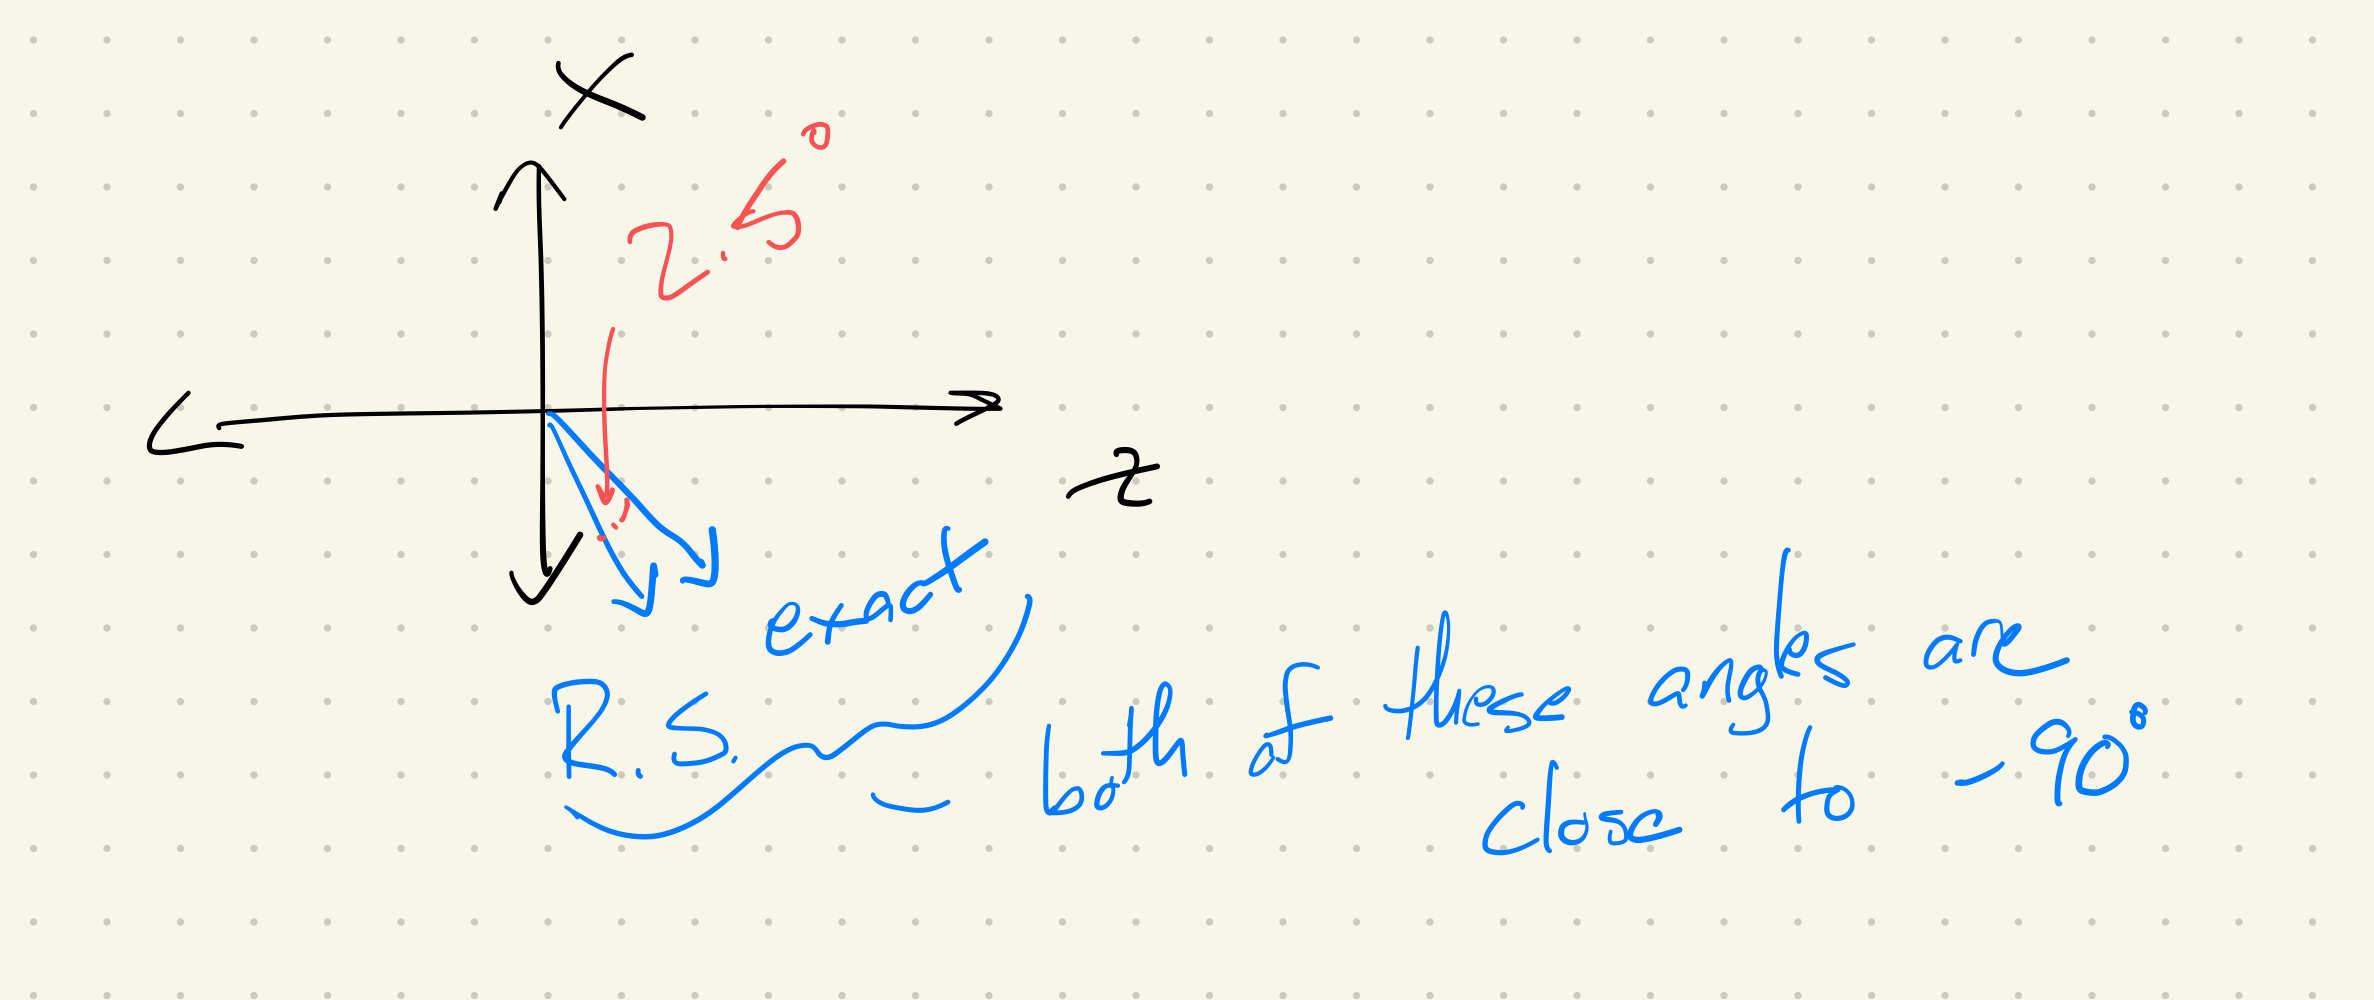
\includegraphics[width=.75\textwidth]{orient-sketch}
  \caption{Sketch of the approximate and exact orientation vectors}
  \label{fig:orient-sketch}
\end{figure}

{\large \textbf{Improved time-stepping and some numerical issues}}

\begin{itemize}
\item I modified the time-stepping code to use a 2nd order explicit
  Runge-Kutta update. There is one difference between my code and a
  standard Runge-Kutta algorithm: I need to re-normalize my
  orientation vector at every step. When I was using forward Euler, I
  just re-normalized at the end of the time step, but with Runge Kutta
  I think it makes sense to renormalize every ``guess'' at the next
  function value. The algorithm I use is the following:
  
  \begin{align*}
    \vect{k}_1 = \vect{\Omega}(\vect{e}_m^i) \times \vect{e}_m^i,
    \qquad \hat{\vect{e}}_m^{i+1} = \vect{e}_m^i + \Delta t \cdot
    \vect{k}_1, \qquad \tilde{\vect{e}}_m^{i+1} =
    \hat{\vect{e}}_m^{i+1} / \|\hat{\vect{e}}_m^{i+1}\| \\ 
    \vect{k}_2 = \vect{\Omega}(\tilde{\vect{e}}_m^{i+1}) \times
    \tilde{\vect{e}}_m^{i+1}, \qquad {\vect{e}_m^\dag}^{i+1} =
    \vect{e}_m^i + \frac{\Delta t}{2} (\vect{k}_1 + \vect{k}_2),
    \qquad \vect{e}_m^{i+1} = {\vect{e}_m^\dag}^{i+1} /
    \|{\vect{e}_m^\dag}^{i+1}\|
  \end{align*}
\item The time-consuming factor here is finding the angular velocities
  $\vect{\Omega}$. This algorithm is globally 2nd order accurate,
  compared to the 1st order accuracy of forward Euler, but requires 2
  regularized Stokeslet solves per time step.
\item From previous numerical experiments, we can estimate the error
  in each RS solve to be roughly 0.01 with 386 nodes, and with
  $4\times$ as many nodes (the spacing between nodes goes down by a
  factor of 2), the error is roughly cut in half. Assuming
  the RS solves are 1st order in the node spacing, matching the RS
  error to the local truncation error gives us a way to choose the
  time step size for a given mesh size on the ellipsoid.
\item For 386 nodes, we are fine with an error of around 0.01 on each
  step. The local truncation error of forward Euler is
  $\mathcal{O}(\Delta t^2)$, so we want to take $\Delta t \sim
  0.1$. For RK2, the local truncation error is $\mathcal{O}(\Delta
  t^3)$ and so if we're using that method we want $\Delta t \sim
  0.22$. However, because each time step incurs twice the work in RK2,
  these two methods are comparable (for this mesh size).
\item When the mesh is finer ($4\times$ as many nodes), RK2 does
  better than forward Euler. For forward Euler we want $\Delta t \sim
  0.0707$ and for RK2 we want $\Delta t \sim 0.171$. For finer meshes,
  RK2 gives bigger improvements over forward Euler.
\item Also as a continuation from last week, I tried to run the
  experiments with an ellipsoid close to the wall (e.g. starting the
  ellipsoid with $\vect{e}_m = \vect{e}_x$ and a distance of
  1). Basically I wanted to extend the experiment shown in Figure
  \ref{fig:third-wall-test} to show a full flip of the
  platelet. However, the integration failed when the surface of the
  ellipsoid overlapped with the wall after one of the time steps.
\item I didn't save any data from this run, so I can only guess what
  happened, but I think my time step must've been too large when the
  ellipsoid got close to the wall.
\item It seems like the fix here is to check at the end of each time
  step that I have a valid orientation, and if I don't, cut the time
  step in half.
\item Interestingly, this only occurred at the finest mesh size, but
  not either of the coarser sizes.
\item I didn't have time to re-run the finest mesh, but I did run a
  long experiment with the coarse mesh and the intermediate mesh and
  plotted results in Figure \ref{fig:long-wall-test} (labeled as the
  ``exact'' solution in the plots).
\end{itemize}

\begin{figure}
  \centering
  \begin{subfigure}{0.49\textwidth}
    \includegraphics[width=\textwidth]{orient_plot13_2nd}
  \end{subfigure}
  \hfill
  \begin{subfigure}{0.49\textwidth}
    \includegraphics[width=\textwidth]{orient_err_plot13_2nd}
  \end{subfigure}
  \\
  \begin{subfigure}{0.49\textwidth}
    \includegraphics[width=\textwidth]{com_plot13_2nd}
  \end{subfigure}
  \caption{Plots of the ellipsoid orientation, orientation error, and
     center of mass in a shear flow near a wall. The height of the
     center of mass is initialized at $1.2$. Orientation is initialized
     at $\vect{e}_m = \vect{e}_x$. }
  \label{fig:long-wall-test}
\end{figure}

% \begin{figure}
%   \centering
%   \begin{subfigure}{0.49\textwidth}
%     \includegraphics[width=\textwidth]{orient_plot11}
%   \end{subfigure}
%   \hfill
%   \begin{subfigure}{0.49\textwidth}
%     \includegraphics[width=\textwidth]{orient_plot16}
%   \end{subfigure}
%   \\
%   \begin{subfigure}{0.49\textwidth}
%     \includegraphics[width=\textwidth]{orient_err_plot11}
%   \end{subfigure}
%   \hfill
%   \begin{subfigure}{0.49\textwidth}
%     \includegraphics[width=\textwidth]{orient_err_plot16}
%   \end{subfigure}
%   \\
%   \begin{subfigure}{0.49\textwidth}
%     \includegraphics[width=\textwidth]{vel_err_plot11}
%   \end{subfigure}
%   \hfill
%   \begin{subfigure}{0.49\textwidth}
%     \includegraphics[width=\textwidth]{vel_err_plot16}
%   \end{subfigure}
%   \caption{Plots of the ellipsoid orientation, orientation error, and
%     velocity error in an unbounded shear flow. Orientation is
%     initialized at $\vect{e}_m = \vect{e}_x$. The three plots in the
%     left column are with the coarse mesh, and the three plots in the
%     right column are with the fine mesh. I didn't plot the center of
%     mass, because it remains constant.}
%   \label{fig:first-free-test}
% \end{figure}

% \begin{figure}
%   \centering
%   \begin{subfigure}{0.49\textwidth}
%     \includegraphics[width=\textwidth]{orient_plot21}
%   \end{subfigure}
%   \hfill
%   \begin{subfigure}{0.49\textwidth}
%     \includegraphics[width=\textwidth]{orient_plot26}
%   \end{subfigure}
%   \\
%   \begin{subfigure}{0.49\textwidth}
%     \includegraphics[width=\textwidth]{orient_err_plot21}
%   \end{subfigure}
%   \hfill
%   \begin{subfigure}{0.49\textwidth}
%     \includegraphics[width=\textwidth]{orient_err_plot26}
%   \end{subfigure}
%   \\
%   \begin{subfigure}{0.49\textwidth}
%     \includegraphics[width=\textwidth]{vel_err_plot21}
%   \end{subfigure}
%   \hfill
%   \begin{subfigure}{0.49\textwidth}
%     \includegraphics[width=\textwidth]{vel_err_plot26}
%   \end{subfigure}
%   \caption{Plots of the ellipsoid orientation, orientation error, and
%     velocity error in an unbounded shear flow. Orientation is
%     initialized at $\vect{e}_m = (1/\sqrt{2}, 1/\sqrt{2}, 0)^T$.}
%   \label{fig:second-free-test}
% \end{figure}

% \begin{figure}
%   \centering
%   \begin{subfigure}{0.49\textwidth}
%     \includegraphics[width=\textwidth]{orient_plot31}
%   \end{subfigure}
%   \hfill
%   \begin{subfigure}{0.49\textwidth}
%     \includegraphics[width=\textwidth]{orient_plot36}
%   \end{subfigure}
%   \\
%   \begin{subfigure}{0.49\textwidth}
%     \includegraphics[width=\textwidth]{orient_err_plot31}
%   \end{subfigure}
%   \hfill
%   \begin{subfigure}{0.49\textwidth}
%     \includegraphics[width=\textwidth]{orient_err_plot36}
%   \end{subfigure}
%   \\
%   \begin{subfigure}{0.49\textwidth}
%     \includegraphics[width=\textwidth]{vel_err_plot31}
%   \end{subfigure}
%   \hfill
%   \begin{subfigure}{0.49\textwidth}
%     \includegraphics[width=\textwidth]{vel_err_plot36}
%   \end{subfigure}
%   \caption{Plots of the ellipsoid orientation, orientation error, and
%     velocity error in an unbounded shear flow. Orientation is
%     initialized at $\vect{e}_m = \vect{e}_y$.}
%   \label{fig:third-free-test}
% \end{figure}

% \begin{figure}
%   \centering
%   \begin{subfigure}{0.49\textwidth}
%     \includegraphics[width=\textwidth]{orient_plot12}
%   \end{subfigure}
%   \hfill
%   \begin{subfigure}{0.49\textwidth}
%     \includegraphics[width=\textwidth]{orient_plot17}
%   \end{subfigure}
%   \\
%   \begin{subfigure}{0.49\textwidth}
%     \includegraphics[width=\textwidth]{orient_err_plot12}
%   \end{subfigure}
%   \hfill
%   \begin{subfigure}{0.49\textwidth}
%     \includegraphics[width=\textwidth]{orient_err_plot17}
%   \end{subfigure}
%   \\
%   \begin{subfigure}{0.49\textwidth}
%     \includegraphics[width=\textwidth]{com_plot12}
%   \end{subfigure}
%   \hfill
%   \begin{subfigure}{0.49\textwidth}
%     \includegraphics[width=\textwidth]{com_plot17}
%   \end{subfigure}
%   \caption{Plots of the ellipsoid orientation, orientation error, and
%     center of mass in a shear flow near a wall. The height of the
%     center of mass is initialized at $1.5$. Orientation is initialized
%     at $\vect{e}_m = \vect{e}_x$. The three plots in the left column
%     are with the coarse mesh, and the three plots in the right column
%     are with the fine mesh.}
%   \label{fig:first-wall-test}
% \end{figure}

% \begin{figure}
%   \centering
%   \begin{subfigure}{0.49\textwidth}
%     \includegraphics[width=\textwidth]{orient_plot13}
%   \end{subfigure}
%   \hfill
%   \begin{subfigure}{0.49\textwidth}
%     \includegraphics[width=\textwidth]{orient_plot18}
%   \end{subfigure}
%   \\
%   \begin{subfigure}{0.49\textwidth}
%     \includegraphics[width=\textwidth]{orient_err_plot13}
%   \end{subfigure}
%   \hfill
%   \begin{subfigure}{0.49\textwidth}
%     \includegraphics[width=\textwidth]{orient_err_plot18}
%   \end{subfigure}
%   \\
%   \begin{subfigure}{0.49\textwidth}
%     \includegraphics[width=\textwidth]{com_plot13}
%   \end{subfigure}
%   \hfill
%   \begin{subfigure}{0.49\textwidth}
%     \includegraphics[width=\textwidth]{com_plot18}
%   \end{subfigure}
%   \caption{Plots of the ellipsoid orientation, orientation error, and
%     center of mass in a shear flow near a wall. The height of the
%     center of mass is initialized at $1.2$. Orientation is initialized
%     at $\vect{e}_m = \vect{e}_x$. The three plots in the left column
%     are with the coarse mesh, and the three plots in the right column
%     are with the fine mesh.}
%   \label{fig:second-wall-test}
% \end{figure}

\begin{figure}
  \centering
  \begin{subfigure}{0.49\textwidth}
    \includegraphics[width=\textwidth]{orient_plot14}
  \end{subfigure}
  \hfill
  \begin{subfigure}{0.49\textwidth}
    \includegraphics[width=\textwidth]{orient_plot19}
  \end{subfigure}
  \\
  \begin{subfigure}{0.49\textwidth}
    \includegraphics[width=\textwidth]{orient_err_plot14}
  \end{subfigure}
  \hfill
  \begin{subfigure}{0.49\textwidth}
    \includegraphics[width=\textwidth]{orient_err_plot19}
  \end{subfigure}
  \\
  \begin{subfigure}{0.49\textwidth}
    \includegraphics[width=\textwidth]{com_plot14}
  \end{subfigure}
  \hfill
  \begin{subfigure}{0.49\textwidth}
    \includegraphics[width=\textwidth]{com_plot19}
  \end{subfigure}
  \caption{Plots of the ellipsoid orientation, orientation error, and
    center of mass in a shear flow near a wall. The height of the
    center of mass is initialized at $1.0$. Orientation is initialized
    at $\vect{e}_m = \vect{e}_x$. The three plots in the left column
    are with the coarse mesh, and the three plots in the right column
    are with the fine mesh.}
  \label{fig:third-wall-test}
\end{figure}

\bibliographystyle{plain}
\bibliography{/Users/andrewwork/Documents/grad-school/thesis/library}

\end{document}




